\section{Génération d'objet paramétrique~: le diamant}

Premièrement nous nous sommes attaqué au maillage des diamants.
L'algorithme se fait donc en deux étapes, la première étant la génération des points dans l'espace.
On considère pour cela deux sommets aux extrémités du diamant, ainsi que 2 cercles sur lesquels
seront répartis un certain nombre de points, dépendamment du nombre de facettes désiré.

{\centering
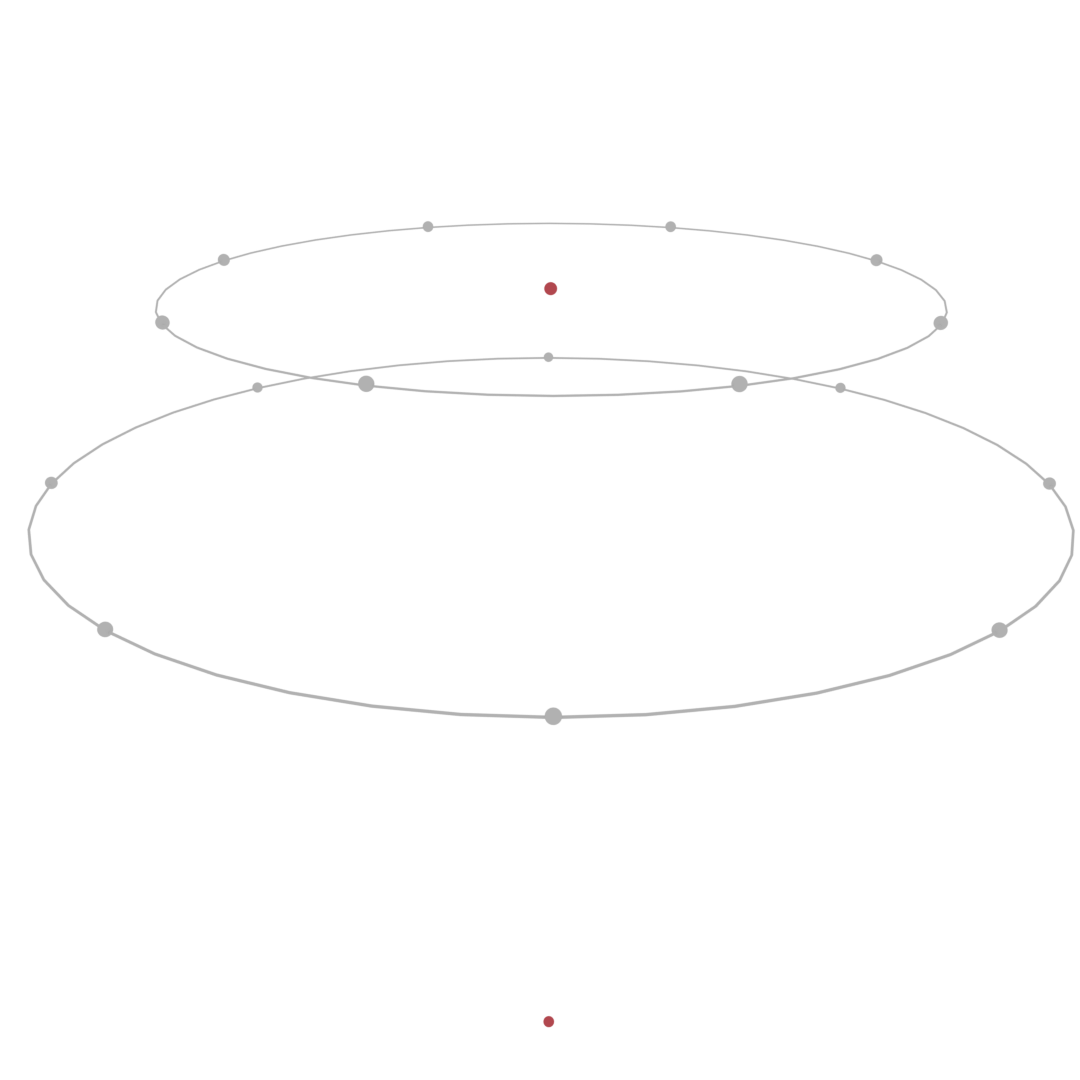
\includegraphics[width=0.7\textwidth]{Maillage/circles}}

Une fois les points placés, il ne reste plus qu'a les relier avec des triangles simples, étant donné
qu'hormis les triangles de la face supérieure, tout les autres triangles auront des normales différentes.

{\centering
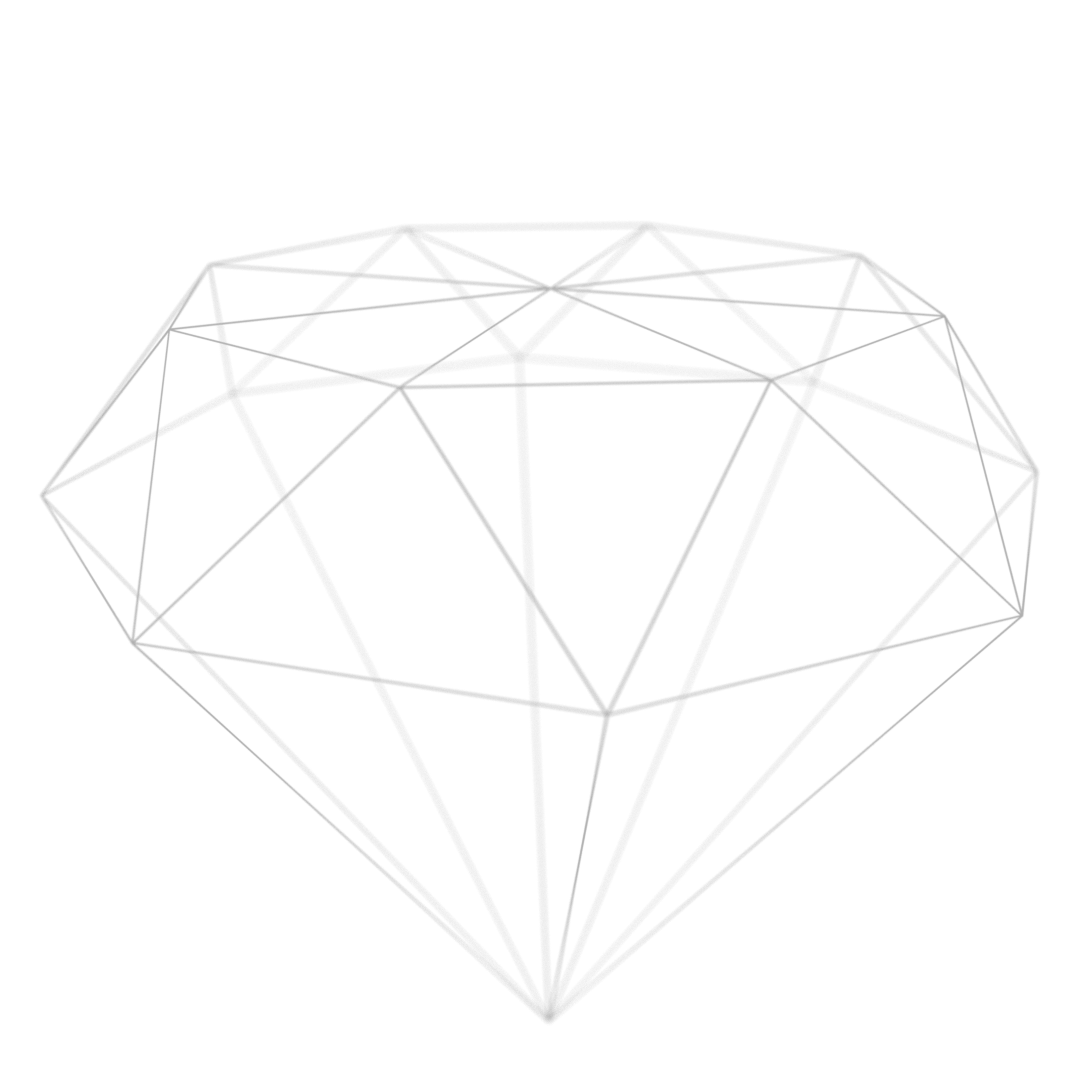
\includegraphics[width=0.7\textwidth]{Maillage/wireframe}}

Il ne reste plus qu'a calculer les normales de chaque face à l'aide d'un produit
vectoriel et en choisissant bien les vecteurs.

La figure suivante montre résultat final avec le système d'éclairage de Phong que nous
allons présenter dans la section précédente~:

{\centering
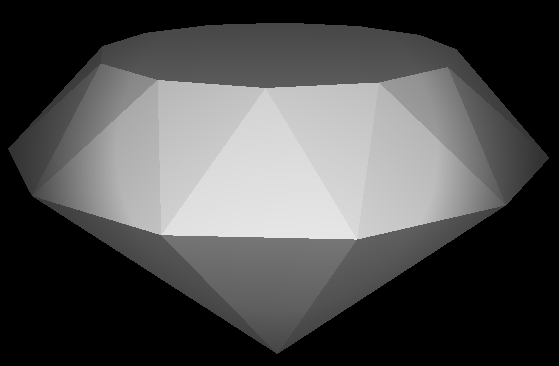
\includegraphics[width=0.7\textwidth]{Maillage/result}}

